% CVPR 2025 Paper Template; see https://github.com/cvpr-org/author-kit

\documentclass[10pt,twocolumn,letterpaper]{article}

%%%%%%%%% PAPER TYPE  - PLEASE UPDATE FOR FINAL VERSION
 \usepackage{cvpr}              % To produce the CAMERA-READY version
% \usepackage[review]{cvpr}      % To produce the REVIEW version
% \usepackage[pagenumbers]{cvpr} % To force page numbers, e.g. for an arXiv version

% Import additional packages in the preamble file, before hyperref
%
% --- inline annotations
%
\newcommand{\red}[1]{{\color{red}#1}}
\newcommand{\todo}[1]{{\color{red}#1}}
\newcommand{\TODO}[1]{\textbf{\color{red}[TODO: #1]}}
% --- disable by uncommenting  
% \renewcommand{\TODO}[1]{}
% \renewcommand{\todo}[1]{#1}



% It is strongly recommended to use hyperref, especially for the review version.
% hyperref with option pagebackref eases the reviewers' job.
% Please disable hyperref *only* if you encounter grave issues, 
% e.g. with the file validation for the camera-ready version.
%
% If you comment hyperref and then uncomment it, you should delete *.aux before re-running LaTeX.
% (Or just hit 'q' on the first LaTeX run, let it finish, and you should be clear).
\definecolor{cvprblue}{rgb}{0.21,0.49,0.74}
\usepackage[pagebackref,breaklinks,colorlinks,allcolors=cvprblue]{hyperref}

%%%%%%%%% PAPER ID  - PLEASE UPDATE
\def\paperID{*****} % *** Enter the Paper ID here
\def\confName{CVPR}
\def\confYear{2025}

%%%%%%%%% TITLE - PLEASE UPDATE
\title{Computer Vision Milestone Report}

%%%%%%%%% AUTHORS - PLEASE UPDATE
\author{Zhengyang Zhang \& Changxun Pan\\
IIIS, Tsinghua University\\
\href{https://iiis.tsinghua.edu.cn}{iiis.tsinghua.edu.cn}\\
{\tt\small zhangzhe24@mails.tsinghua.edu.cn \& pcx24@mails.tsinghua.edu.cn}
% For a paper whose authors are all at the same institution,
% omit the following lines up until the closing ``}''.
% Additional authors and addresses can be added with ``\and'',
% just like the second author.
% To save space, use either the email address or home page, not both
}

\begin{document}
\maketitle
%\begin{abstract}
The ABSTRACT is to be in fully justified italicized text, at the top of the left-hand column, below the author and affiliation information.
Use the word ``Abstract'' as the title, in 12-point Times, boldface type, centered relative to the column, initially capitalized.
The abstract is to be in 10-point, single-spaced type.
Leave two blank lines after the Abstract, then begin the main text.
Look at previous \confName abstracts to get a feel for style and length.
\end{abstract}    
\section{Introduction}
Emotion recognition represents a critical frontier in computer vision, enabling machines to interpret human facial expressions—one of our most fundamental forms of non-verbal communication. This capability is essential for developing truly intuitive human-computer interfaces and responsive robotic systems.\\

This project addresses the challenge of real-time emotion recognition on resource-constrained platforms. While powerful deep learning models can achieve impressive accuracy, they often require substantial computational resources incompatible with edge devices. We focus on developing efficient algorithms that maintain high accuracy while operating in real-time on standard laptops with integrated GPUs or even smartphones.\\

Our approach combines optimized face detection techniques with lightweight convolutional neural networks, complemented by several performance-enhancing optimizations. We demonstrate that our system achieves accuracy comparable to trained humans while maintaining processing speeds suitable for real-time applications.
\section{Problem Statement}
\subsection{Readings to be examined}
There are many prior works that are related to face detection and emotion detection. We need the algorithm for face detection as the input of our problem is not a single portrait, but a full scene photograph in different scenarios. Therefore, before we can judge the emotion, we need to first find the faces and crop them down for further emotion detection. In this point of view, we need to read some of the paper regarding face detection and marking, for example ``ASFD: Automatic and Scalable Face Detector"\cite{ASFD}. We also need to read some of the papers on image classification, for example ``EfficientNet: Rethinking Model Scaling for Convolutional Neural Networks"\cite{EfficientNet}, especially those that have a smaller number of parameters and shallower network structure, which may help to reduce the inference cost, thus, helping to reach the goal of fast and efficient emotion recognition.

\subsection{Dataset to be used}
There are some face emotion recognition dataset on the Internet, for example, the ``Facial Emotion Recognition Dataset" contains lots of pictures tagged with seven different emotions, we can use this data to train the model. In addition, we also need some data to train face detection. We found ``Face-Detection-Dataset" on kaggle, which contains ``16.7k images and 2 annotation files". 

\subsection{Core Method or algorithm}
We will divide this task into 2 parts, the first is face detection, we can use different kernel size to scan through the image an run a neural network to tell whether there is a face in the kernel, which can help us find the place of the face. Then we can crop the face down and send this partial image into a another neural network, then we can  use this neural network to tell the emotion.

When running inference, we can still follow this pipeline, before sending the picture into neural network, we can first run max pool or average pool to blur the image, which can help to reduce the amount of calculation needed.

In addition, we can also choose different precisions of the parameters. Smaller precision of the parameters does not necessarily cause the accuracy to reduce, but it must reduce the amount of calculation needed.

\subsection{The method of evaluating results}
There are several ways to evaluate. 

First, we can divide the data set into a training set and an evaluation set to partially test the accuracy of the neural network. Inference speed can also be tested.

Second, we can shot some videos in real life and compare the result with the real emotion. The videos can be in different resolution, and can be of different distance to the human, which can test the robustness of the algorithm and neural network. Also, the fast frame rate of real-life videos can also test the efficiency of the algorithm.

Our final goal is to implement this algorithm on laptops with only integrated GPU or even on smartphones. So, the final test is try to move this program onto smartphones and try to use smatrphones' cameras to detect emotion in real life.

\section{Technical approach}
The main techniques for this problem can be described as follows
\begin{enumerate}
		\item \textbf{Face detection and landmark localization:} We employ dlib's face detection model, which utilizes Histogram of Oriented Gradients (HOG) features and a Support Vector Machine (SVM) classifier to locate faces in images. The system further identifies 68 facial landmarks corresponding to key facial features, establishing the foundation for emotion analysis.
		\item \textbf{Emotion classification:} We implement a Convolutional Neural Network (CNN) based on the ResNet-18 architecture to classify facial expressions into distinct emotional categories. We evaluate the model's performance against human benchmarks to validate its effectiveness, as emotion recognition is a challenging task even for humans.
\end{enumerate}
In this process, there may be some difficulties, especially in terms of efficiency. As the neural network is very computationally costly, we have to think of some methods to reduce time consumption.

The ways we thought of can be described as follows:
\subsection{Efficiency promotion}
\begin{enumerate}
    \item \textbf{Localized detection:} We know that the face can not move very fast in the picture, so we can just detect a small area around the position of faces in the last frame. We detect on the global scale only if there is no face in the last frame. You may wonder what if the scope changed suddenly, it doesn't matter. In the first frame after changing the scope, we cannot detect the face, but after that, we will find that there is no face in the last frame, and then detection on a global scale will be done. So, indeed, we may lose at most one frame, which cannot be observed.
    \item \textbf{Reduced resolution scanning:} some computation can be saved when scanning the whole picture. We can just reduce the resolution of the picture by several times, as we just need to find the position of the faces, very high resolution is not necessary. For example, we find that 480P is good enough than 1080P. The model can still find the face in 480P, and the time consumption is much less than that in 1080P.
    \item \textbf{Dynamic resolution adjustment:} when the face is very large, we can also reduce the resolution, as it is just about finding the face.
\end{enumerate}
\subsection{CNN recognition}
We observed that the data distribution was highly unbalanced, with the disgust class being significantly underrepresented while the happy class was overrepresented. To address this issue, we applied data augmentation techniques to balance the class distribution. This preprocessing step improved our classification results, particularly for the rare emotion categories that would otherwise have been difficult to recognize accurately.

We employed a ResNet architecture for emotion classification. Notably, facial expression classification is challenging even for humans. To establish a benchmark, we conducted experiments with human participants (our classmates). Initially, they achieved approximately 40\% accuracy, and even after extensive exposure to the dataset, their performance plateaued at around 65\%. Our model achieved an average test accuracy of 62\% (Figure \ref{fig:test_acc}), which is comparable to human performance on this challenging task.

\begin{figure}[!htb]
	\centering
	 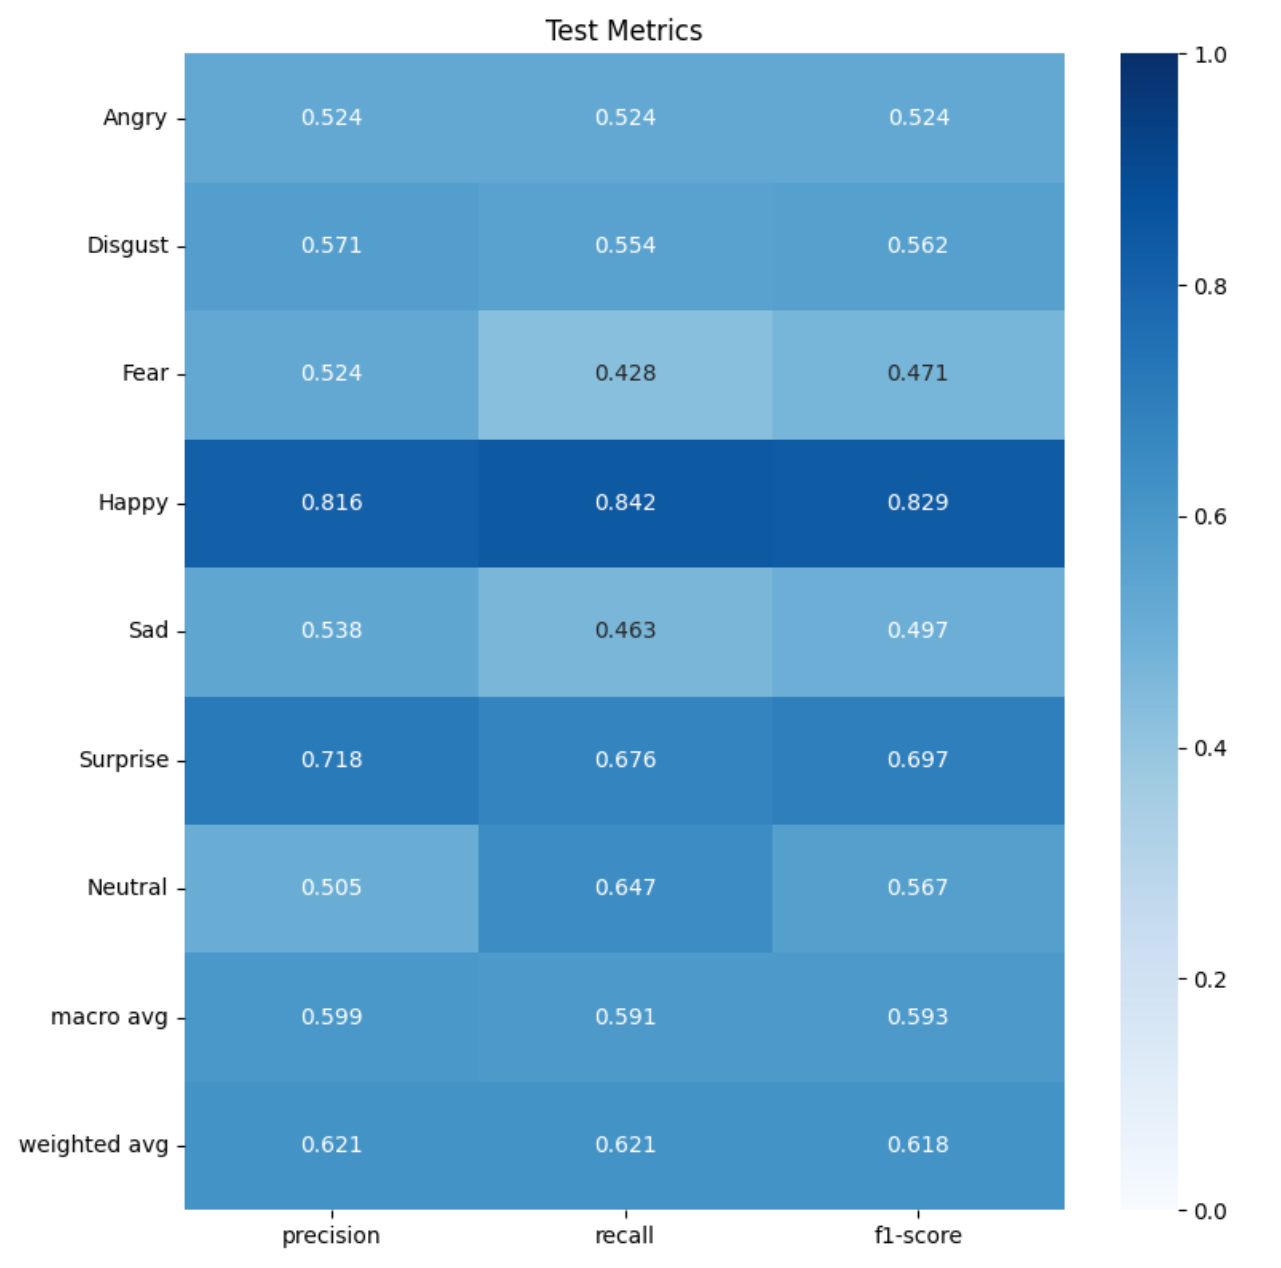
\includegraphics[width=1.0\linewidth]{sec/assets/test_acc.png}
	 \caption{The model achieved 62\% accuracy on the test set, comparable to trained human performance.}
	 \label{fig:test_acc}
\end{figure}


\section{Intermediate Results}
\subsection{Test Dataset}
We used a standard video of 2 minutes and 18 seconds at 30fps for testing. The video typically featured 1-3 people. All experiments were conducted on a laptop CPU. For efficiency, we processed every other frame and copied the results to adjacent frames, as facial expressions change minimally between consecutive frames. A 1080P video served as our initial test case.

\subsection{Implementation Time}
First, we tested a nearly 1080P video without optimization. The naive pipeline, which detected faces and classified emotions in each frame, took 7m26s to complete (Figure \ref{fig:original_command}), which was prohibitively long for practical use.
\begin{figure}[!htb]
	\centering
	 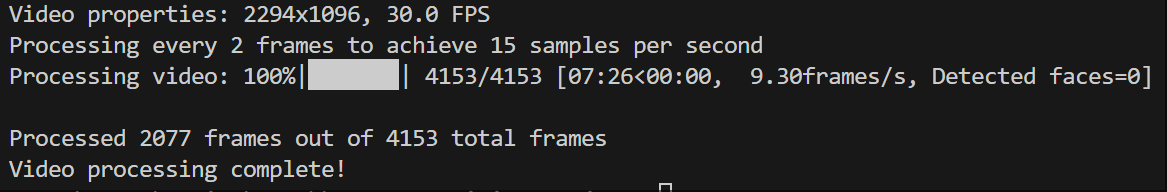
\includegraphics[width=1.0\linewidth]{sec/assets/original_command.png}
	 \caption{Original run with the naive pipeline: processing time was 7m26s.}
	 \label{fig:original_command}
\end{figure}

We tested multiple video resolutions to optimize processing speed. Our experiments showed that while high-resolution videos are not essential for effective face and emotion detection, excessively low resolution leads to detection failures. Testing demonstrated that 480P provided the optimal balance between accuracy and performance, reducing processing time to just 1m38s (Figure \ref{fig:480P_command}). Based on these findings, we implemented automatic resolution adjustment to approximately 480P for all subsequent experiments.
\begin{figure}[!htb]
	\centering
	 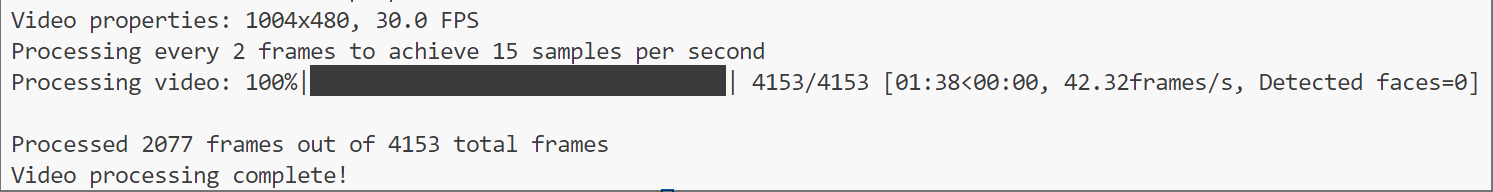
\includegraphics[width=1.0\linewidth]{sec/assets/480P_command.png}
	 \caption{The 480P video required only 1m38s to process.}
	 \label{fig:480P_command}
\end{figure}

A key optimization involved implementing local detection: examining only the area surrounding the previous frame's face location, unless no face was detected. We tested various padding sizes, with pad dynamically defined as: $\text{pad} = \max(30, \text{int}(\text{p} \cdot \max(\text{face\_width}, \text{face\_height})))$. Figure \ref{fig:pad_size} presents our experimental results. We selected p=1.0 as the optimal trade-off between processing speed and detection accuracy.

We also implemented dynamic resolution adjustment based on face size. When the face-to-image size ratio fell below a threshold (while maintaining sufficient resolution of at least 96$\times$96 pixels for reliable emotion detection), we downscaled the image by a factor of 2. The scaling parameter reset whenever no face was detected in the previous frame. With p=1.0, this optimization further reduced processing time to 1m10s (Figure \ref{auto_face_command}), showing promising potential for real-time applications.

\begin{figure}[!htb]
\centering
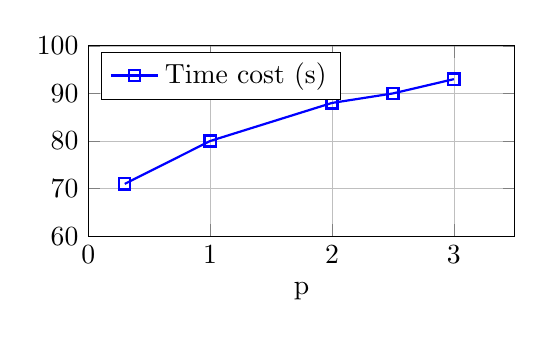
\begin{tikzpicture}
\begin{axis}[
	width=7cm,
	height=4cm,
	xlabel={p},
	ylabel={},
	xmin=0, xmax=3.5,
	ymin=60, ymax=100,
	xtick={0,1,2,3},
	ytick={60,70,80,90,100},
	legend pos=north west,
	grid=both,
	grid style={line width=.05pt, draw=gray!10},
	major grid style={line width=.2pt,draw=gray!50}
]
\addplot[mark=square,blue,thick] coordinates {
	(0.3,71)
	(1.0,80)
	(2.0,88)
		(2.5,90)
		(3.0,93)
};
\legend{Time cost (s)}
\end{axis}
\end{tikzpicture}
\caption{Processing time with different pad sizes. The pad size is dynamically defined as: $\text{pad} = \max(30, \text{int}(\text{p} \cdot \max(\text{face\_width}, \text{face\_height})))$. Global detection alone would require approximately 100s.}
\label{fig:pad_size}
\end{figure}

\begin{figure}[!htb]
	\centering
	 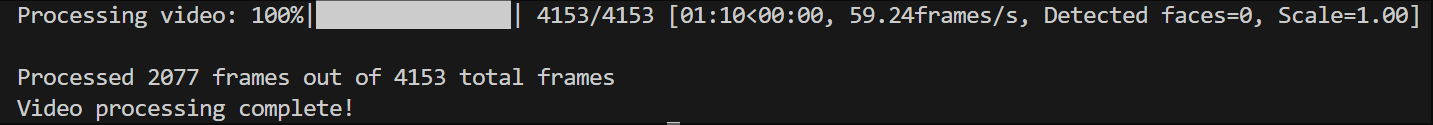
\includegraphics[width=1.0\linewidth]{sec/assets/auto_face_command.png}
	 \caption{Automatic face resolution adjustment reduced processing time to 1m10s.}
	 \label{auto_face_command}
\end{figure}

\subsection{Recognition Accuracy}
As mentioned previously, untrained humans achieve approximately 40\% accuracy in emotion recognition, while trained humans reach about 60\%. Our model achieved 62\% accuracy, comparable to trained human performance.

\subsection{Result Demonstration}
Figure \ref{fig:jg_exp} demonstrates our emotion detection system in action. The model successfully identified both faces and correctly classified their emotions as "happy."

\begin{figure}[!htb]
	\centering
	 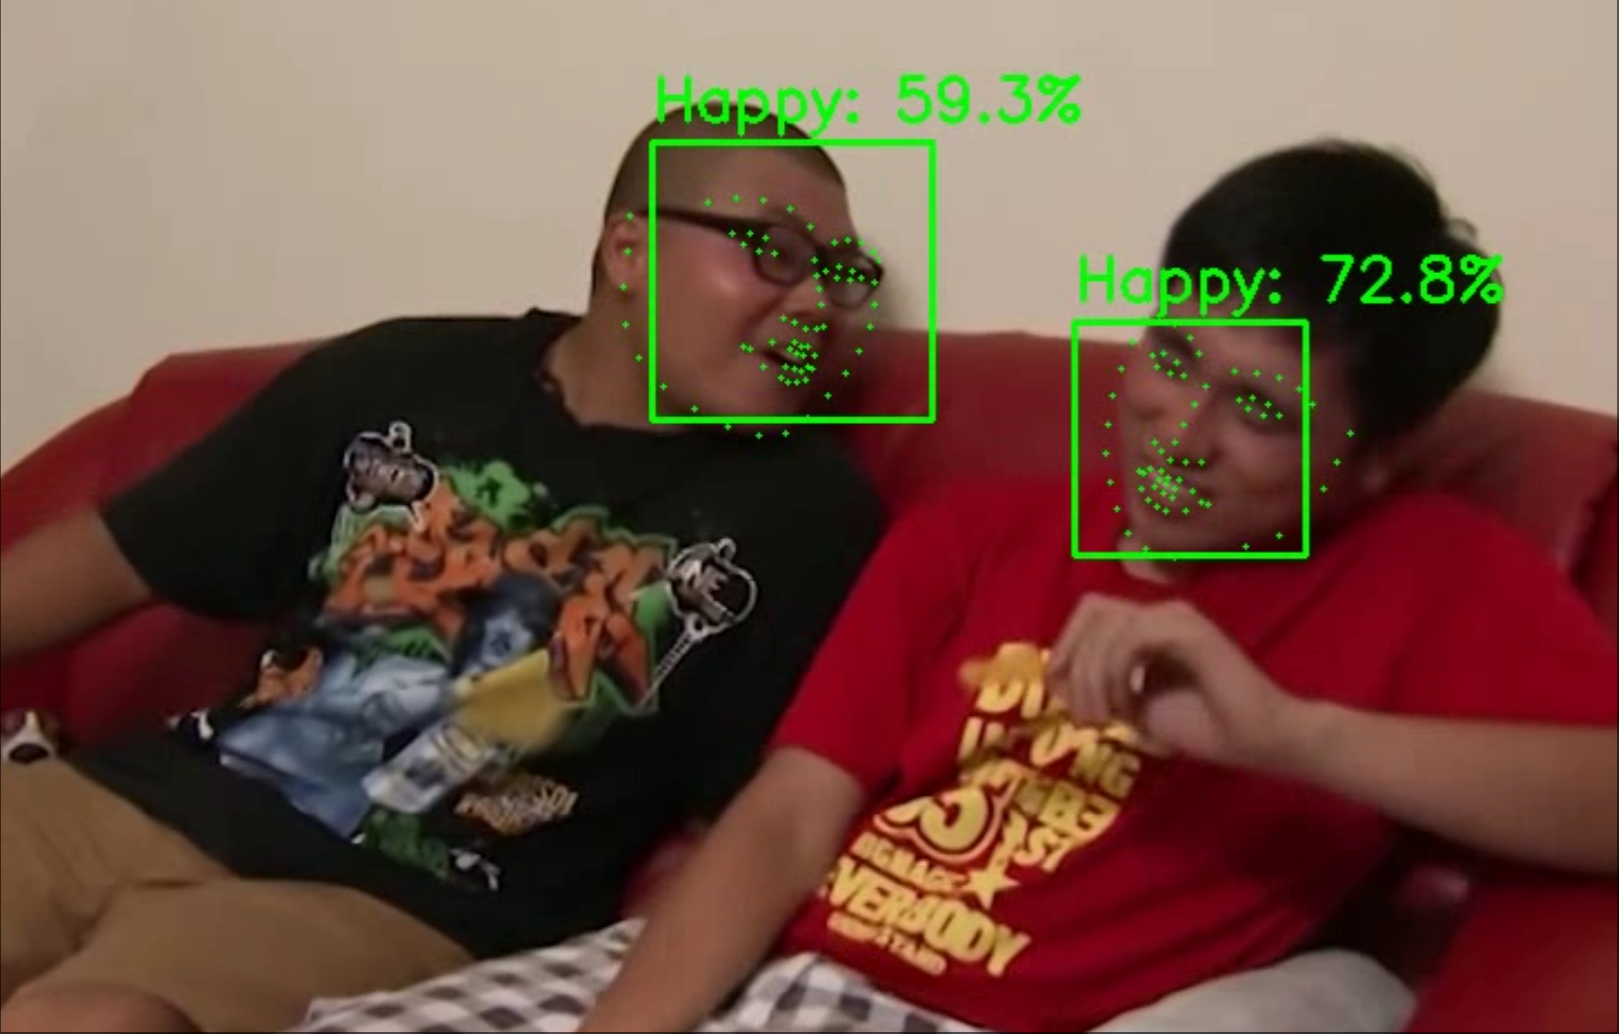
\includegraphics[width=0.8\linewidth]{sec/assets/jg_exp.png}
	 \caption{Example of emotion detection. The model successfully recognizes two faces and correctly identifies both emotions as "happy."}
	 \label{fig:jg_exp}
\end{figure}

The video processing time of approximately 1 minute and 10 seconds enabled analysis at nearly 24 frames per second, making it suitable for real-time applications.

\section{Future work}
\subsection{Distorted face detection}
In a video, faces are in different poses, which may cause problems for detection. Actually, in experiments, the model failed to detect the distorted faces. We also consider using a stronger model to fix this problem, however, it may cost a lot. 
So in order to let the model work properly, we need to transform the face back to the right position. We can use SIFT for this function. The eyes and edge of the lips are often keypoints, and as the model for finding the faces actually detect the eyes and lips, we can just select these points as the keypoint and further detect it. 
Then we can use homography transformation to find the original picture of the distorted faces and then use the model to detect the position of the face. 
	
{
    \small
    \bibliographystyle{ieeenat_fullname}
    \bibliography{main}
}

% WARNING: do not forget to delete the supplementary pages from your submission 
% \clearpage
\setcounter{page}{1}
\maketitlesupplementary


\section{Rationale}
\label{sec:rationale}
% 
Having the supplementary compiled together with the main paper means that:
% 
\begin{itemize}
\item The supplementary can back-reference sections of the main paper, for example, we can refer to \cref{sec:intro};
\item The main paper can forward reference sub-sections within the supplementary explicitly (e.g. referring to a particular experiment); 
\item When submitted to arXiv, the supplementary will already included at the end of the paper.
\end{itemize}
% 
To split the supplementary pages from the main paper, you can use \href{https://support.apple.com/en-ca/guide/preview/prvw11793/mac#:~:text=Delete%20a%20page%20from%20a,or%20choose%20Edit%20%3E%20Delete).}{Preview (on macOS)}, \href{https://www.adobe.com/acrobat/how-to/delete-pages-from-pdf.html#:~:text=Choose%20%E2%80%9CTools%E2%80%9D%20%3E%20%E2%80%9COrganize,or%20pages%20from%20the%20file.}{Adobe Acrobat} (on all OSs), as well as \href{https://superuser.com/questions/517986/is-it-possible-to-delete-some-pages-of-a-pdf-document}{command line tools}.

\end{document}
